\documentclass[a4paper,11pt]{article}
\usepackage[utf8]{inputenc}
\usepackage[spanish]{babel}
\usepackage{fancyhdr}
\usepackage[pdftex]{graphicx}

\newenvironment{scaption}[1]{\caption{{\small #1}}}{}

\newenvironment{desig}{\begin{list}{}{\setlength{\labelsep}{0cm}\setlength{\labelwidth}{0cm}\setlength{\listparindent}{0cm}\setlength{\rightmargin}{\leftmargin}}}{\end{list}}


\author{Pablo Rodriguez Monetti}
\title{Estructura Física del Sistema FG-Tester}
\date{2007}

\begin{document}
 \maketitle
\paragraph{}
El sistema FG-Tester fue desarrollado sobre una arquitectura Cliente-Servidor, con la intención de aprovechar de manera eficiente los recursos provistos por una red de computadoras. Por un lado, lo que se persigue es obtener mayor performance ejecutando varias tareas en paralelo. Por otro, poder correr más de un cliente del FG-Tester en distintas terminales, donde todos ellos consultan a un único repositorio de datos.
Las aplicaciones del sistema FG-Tester (clientes y servidores) pueden dividirse en capas físicas de acuerdo a la topología física de la red de la corporación, teniendo en cuenta que debe haber un único servidor de datos, uno o más servidores de cálculo y uno o más clientes del sistema. Es importante destacar que aunque el sistema fue pensado para ser distribuído, tanto servidores como clientes pueden, eventualmente, correr en una misma computadora.

Dado que todas las aplicaciones del sistema requieren hardware con prestaciones similares, la red estará compuesta solo por PC's de aproximadamente el mismo potencial. Por lo tanto, consideramos que la Estructura de Hardware consta de una única capa.

La Estructura Física, también llamada Estructura de Despliegue, permite relacionar elementos de software con plataformas de ejecución. La relación que usaremos para documentar esta vista es $ALOJADO\_EN$, que en nuestro caso vinculará procesos con procesadores o computadoras. En los siguientes esquemas se ven representadas estas relaciones, teniendo en cuenta que los nodos (denotados con rectángulos) son computadoras, los arcos conexiones de red y en cada nodo se dibujan los procesos alojados en esa computadora. Las agrupaciones de computadores se grafican a través de rectángulos redondeados. Las restricciones matemáticas en cada caso indican la necesidad de tener al menos un servidor de cálculo y al menos un cliente corriendo en alguna computadora, así como la imposibilidad de tener un mismo cliente o un mismo servidor de cálculo corriendo en más de una computadora. Además, las conexiones de red entre los equipos (líneas continuas en los esquemas) deben asegurar que el servidor de datos pueda comunicarse con al menos un servidor de cálculo y un cliente, y que a su vez éstos estén conectados entre sí.


\begin{figure}
\begin{center}
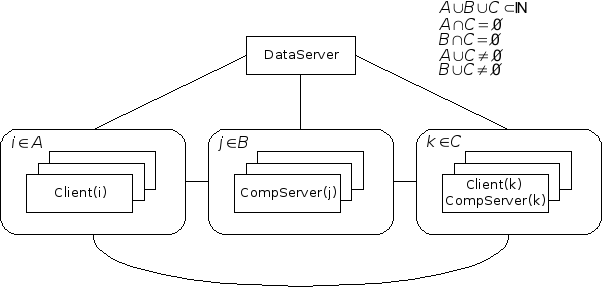
\includegraphics[scale=0.7]{./EstructuraFisica01.png}
\end{center}
\caption{Distribución de procesos en hardware donde el proceso correspondiente al servidor de datos (DataServer) corre de forma solitaria en una computadora.}
\end{figure}


\begin{figure}
\begin{center}
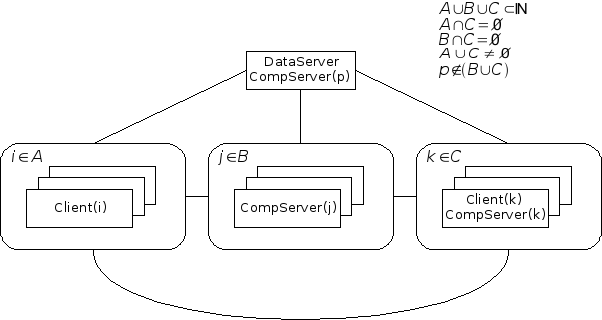
\includegraphics[scale=0.7]{./EstructuraFisica02.png}
\end{center}
\caption{Distribución de procesos en hardware donde el proceso correspondiente al servidor de datos (DataServer) corre junto a un servidor de cálculo (CompServer) en una computadora.}
\end{figure}


\begin{figure}
\begin{center}
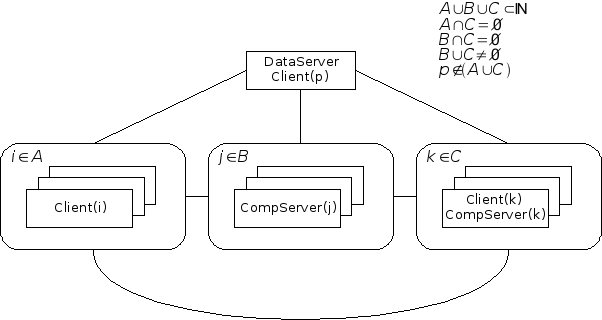
\includegraphics[scale=0.7]{./EstructuraFisica03.png}
\end{center}
\caption{Distribución de procesos en hardware donde el proceso correspondiente al servidor de datos (DataServer) corre junto a un cliente (Client) en una computadora.}
\end{figure}


\begin{figure}
\begin{center}
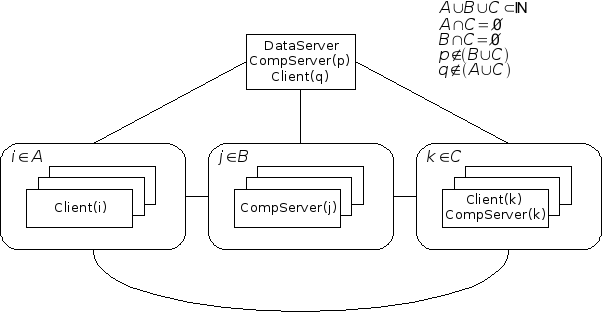
\includegraphics[scale=0.7]{./EstructuraFisica04.png}
\end{center}
\caption{Distribución de procesos en hardware donde el proceso correspondiente al servidor de datos (DataServer) corre junto a servidor de cálculo (CompServer) y a un cliente (Client) en una computadora.}
\end{figure}


\begin{figure}
\begin{center}
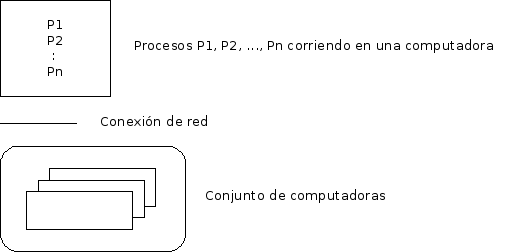
\includegraphics[scale=0.7]{./EstructuraFisica00.png}
\end{center}
\caption{Referencias.}
\end{figure}

\end{document}
